\chapter{Analisi dei requisiti}
Si vuole realizzare un database atto al supporto e alla gestione del personale di controllo del traffico aereo.
\section{Intervista}
Un primo testo ottenuto dall'intervista è il seguente (Estrema semplificazione rispetto ad un caso reale):\\
Si richiede di creare uno strumento che permetta di allocare i turni di lavoro delle rispettive posizioni. La giornata è suddivisa in 3 turni da 8 ore (8:00, 16:00, 24:00), dopo ogni turno lavorativo un controllore deve avere almeno 3 turni di riposo prima di tornare al lavoro, per un massimo di 300 turni annuali.
Esistono 3 tipi di posizioni, ognuna relativa ad un segmento della tratta di volo diverso. 
\begin{itemize}
    \item Aerodromo:
I punti di partenza e di arrivo delle tratte, ogni aerodromo ha una o più piste. %e una o più posizioni di tipo (Delivery, si occupa di fornire clearance IFR; Ground, si occupa di gestire traffico al suolo; Tower, si occupa di gestire gli aeromobili sulle piste.)
\item Avvicinamento:
Sono posizioni il cui compito è di instradare il traffico negli ultimi e nei primi tratti di volo. Creando ove necessario sequenze\footnote{Numero di aerei in "fila" a distanza prestabilita} di traffico.
\item En-Route:
la cui attività è di risolvere conflitti tra le rotte degli aeromobili in fase di crociera, facendoli virare o aumentandone o abbassandone la quota di volo.
\end{itemize}
% image route
\begin{figure}[H]
  \centering
  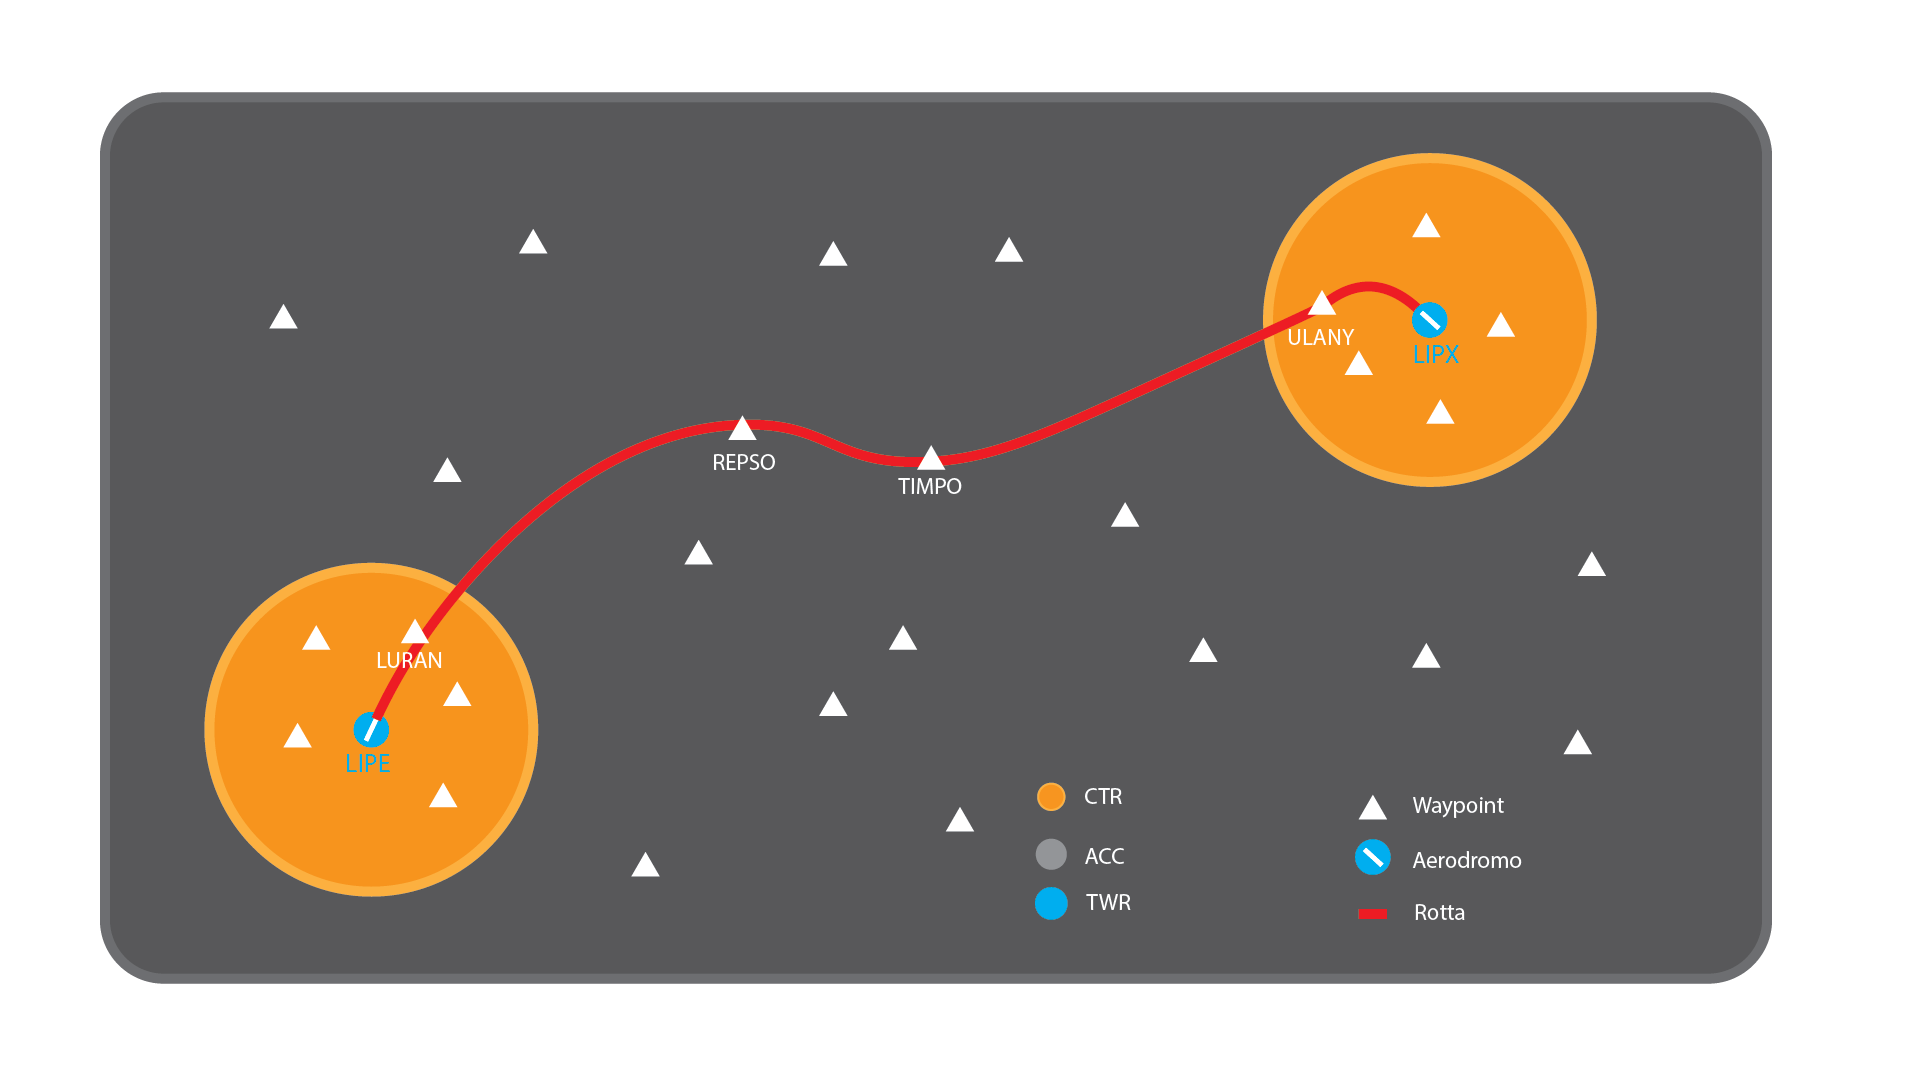
\includegraphics[width=1\textwidth]{figures/Rotta.png}
  \caption{"Un esempio di una rotta e dei settori attraversati"}
\end{figure}
Ogni posizione è contenuta all'interno di un Centro, e ogni posizione contiene uno o più settori, un settore è uno spazio aereo contenente dei waypoint. Durante tutti i turni ogni settore deve essere coperto. 
Ogni posizione ha una capacità massima data dal fatto che un controllore è in grado di gestire uno spazio aereo limitato, quindi le posizioni che contengono più settori avranno una capacità inferiore rispetto a quelle che ne contengono di meno (i settori possono essere raggruppati o divisi al fine di spartire il carico di lavoro tra più posizioni).
Ogni controllore è autorizzato a lavorare solamente in posizioni contenenti settori per i quali ha l’abilitazione, ogni abilitazione è relativa ad uno o più settori ed è individuale. Inoltre possono essere allocati turni al controllore solamente in posizioni appartenenti al centro in cui lavora.
Esistono due tipi di turni, Il primo, di lavoro mentre il secondo di standby, quest'ultimo è necessario per garantire ridondanza, in caso di imprevisti (e.g. controllore malato, traffico eccessivo)
per ogni 3 turni di lavoro è necessario un lavoratore che copre il turno in standby. Occorre tenere uno storico dei turni e dei relativi compensi per computare il RAL a fine anno.
Ogni traffico aereo deve compilare un piano di volo almeno 3 ore prima della partenza (Anche se la maggior parte dei traffici è schedulata con molti mesi di anticipo), ogni piano di volo contiene l'aeromobile che verrà utilizzato (identificato univocamente dal suo numero di coda, simle ad una targa, dove la prima lettera indica la nazionalità di immatricolazione, questo appartiene ad un modello o tipo identificato da massimo 4 caratteri alfanumerici), l'aerodromo di partenza, quello di arrivo e la lista di waypoint che attraverserà con i relativi orari stimati. Ogni aeroporto contiene delle piste il cui numero è dato dall'arrotondamento delle prime due cifre del loro orientamento magnetico (e.g. orientamento 321° la pista sarà 32, mentre dall'altro lato 14) con l'aggiunta di L(left), R(right), o C(center) per piste parallele. Ogni aeroporto contiene anche una o più settori di tipo torre, senza quindi waypoint. 
Ogni punto (i.e. waypoint) appartiene ad un settore di tipo avvicinamento o di rotta.
Ogni controllore ha diritto a 30 giorni di ferie all'anno.\\
Il software deve permettere la gestione dei controllori di volo in termini amministrativi (aggiungere, licenziare, modificare), 
ma ancora più importante è il punto di vista logistico, ogni mese, per il successivo, verranno computati i turni, in modo da riempire tutti i settori facendo lavorare i controllori in maniera equa e selezionando le posizioni attive in modo che non venga mai superata l'occupazione limite delle posizioni (calcolando il traffico previsto sulla posizione al momento del turno).\\
Il secondo software dovrà permettere la gestione di una posizione di aerodromo dando la possibilità di segnare gli aerei in partenza e in arrivo come decollati o atterrati una volta che ciò avviene.\\
Il terzo software dovrà fornire al supervisore del centro un overview riguardo l'occupazione prevista a breve termine (poche ore successive), e dovrà permettergli di cambiare le posizioni aperte, modificando quindi anche i turni.\\
\section{Rilevamento delle ambiguità e correzioni proposte}

Dalla descrizione fornita emergono alcuni punti ambigui o che necessitano di ulteriori specifiche. Di seguito vengono elencati tali punti e vengono proposte delle correzioni o dei chiarimenti per migliorare la comprensione del sistema richiesto.

\begin{enumerate} 
  \item \textbf{Tipi di posizioni}: Si menzionano tre tipi di posizioni (aerodromo, avvicinamento, en-route), ma non viene specificato se un controllore può essere assegnato a una sola posizione o se può coprire più tipi di posizioni.
  
  \item \textbf{Capacità massima delle posizioni}: Viene menzionato che ogni posizione ha una capacità massima determinata dalla capacità di gestione dello spazio aereo da parte di un controllore. Tuttavia, non viene specificato come venga calcolata questa capacità né come venga determinato il numero di settori che una posizione può contenere.
  
  \item \textbf{Turni di lavoro e standby}: Viene menzionato che ci sono due tipi di turni, il primo di lavoro e il secondo di standby. Tuttavia, non viene specificato come vengono assegnati i turni di standby né quali siano le regole per la distribuzione tra i controllori. Inoltre, non viene chiarito se i turni di standby sono obbligatori per tutti i controllori o solo per alcuni.
    
  \item \textbf{Gestione dei controllori di volo}: Viene menzionato che il software deve permettere la gestione amministrativa dei controllori di volo (aggiunta, licenziamento, modifica), ma non viene specificato quali siano le informazioni associate a un controllore e come vengano gestiti i dati personali.
  
  \item \textbf{Gestione dei turni}: Viene menzionato che ogni mese vengono computati i turni per il mese successivo, ma non viene specificato come avviene questo calcolo e quali criteri vengono seguiti per assegnare i turni ai controllori. Inoltre, non viene chiarito se esistono vincoli specifici (ad esempio, giorni di riposo consecutivi) che devono essere rispettati durante la generazione dei turni.
  
  \item \textbf{Software per la gestione di una posizione di aerodromo}: Viene menzionato che deve essere creato un software per la gestione di una posizione di aerodromo, ma non viene specificato quali siano le funzionalità richieste per questo software e quali dati devono essere monitorati.
  
  \item \textbf{Overview dell'occupazione prevista}: Viene menzionato che il supervisore del centro deve avere un'overview riguardo all'occupazione prevista a breve termine e deve poter modificare le posizioni aperte e i turni. Tuttavia, non viene specificato come viene generata questa overview e quali informazioni specifiche deve fornire. Inoltre, non viene chiarito come vengano effettuate le modifiche ai turni e alle posizioni aperte.
  \end{enumerate}

Di seguito vengono fornite soluzioni e correzioni corrispondenti ai punti ambigui e alle specifiche mancanti emersi durante l'analisi dei requisiti.

\begin{enumerate}
\item \textbf{Tipi di posizioni}: È possibile consentire ai controllori di coprire più tipi di posizioni, consentendo loro di avere abilitazioni diverse per gestire le diverse posizioni. In questo modo, un controllore potrà essere assegnato a più posizioni di controllo, a seconda delle loro abilitazioni. Nonostante, generalmente, un centro possiede posizioni di un unico tipo.

\item \textbf{Capacità massima delle posizioni}: Per calcolare la capacità massima delle posizioni, potrebbe essere necessario stabilire un limite superiore di settori che un controllore può gestire efficacemente. In base a questa informazione, sarà possibile determinare la capacità massima di ciascuna posizione in termini di numero massimo di settori che può contenere. Sarà inoltre necessario valutare la complessità dei settori e il carico di lavoro associato per una migliore stima della capacità. Questo studio è stato fatto da esperti e emerge che ad ogni posizione corrisponde una capacità di base = 100 la quale verrà divisa per \[  3^{num-settori-in-posizione} \].

\item \textbf{Turni di lavoro e standby}: È necessario definire le regole per l'assegnazione dei turni di standby ai controllori. Ad esempio, potrebbe essere definito un criterio rotativo in modo che ogni controllore abbia un turno di standby ogni tot turni di lavoro. Inoltre, sarà necessario specificare se i turni di standby sono obbligatori per tutti i controllori o solo per alcuni. Viene comunicato che i turni standby devono essere allocati come quelli standard, in base ai controllori che hanno lavorato meno.

\item \textbf{Gestione dei controllori di volo}: Il sistema deve fornire funzionalità di gestione amministrativa per i controllori di volo. Ciò potrebbe includere la possibilità di aggiungere, licenziare e modificare le informazioni dei controllori nel database. Dovrebbero essere registrati i dati personali dei controllori, le abilitazioni, i giorni di ferie e altre informazioni pertinenti per la gestione del personale.

\item \textbf{Gestione dei turni}: Il calcolo dei turni potrebbe essere basato su algoritmi di scheduling che prendono in considerazione le abilitazioni dei controllori, le capacità delle posizioni e i requisiti di riposo. Potrebbero essere definiti vincoli specifici da rispettare durante la generazione dei turni, ad esempio limiti massimi di turni di lavoro consecutivi o minimi giorni di riposo tra i turni. Sarà necessario definire tali regole e algoritmi per garantire una distribuzione equa dei turni e il rispetto delle normative di lavoro.

\item \textbf{Software per la gestione di una posizione di aerodromo}: Il software per la gestione di una posizione di aerodromo dovrebbe consentire di segnare gli aerei in partenza e in arrivo come decollati o atterrati, indicando l'orario in cui ciò avviene, tenendo traccia delle informazioni relative a ciascun volo. Potrebbe essere utile avere una funzionalità per monitorare lo stato dei voli in tempo reale.

\item \textbf{Overview dell'occupazione prevista}: Il software per il supervisore del centro dovrebbe fornire un'overview dell'occupazione prevista a breve termine, basata sui turni e sulle posizioni assegnate. Potrebbe essere creato un modulo in cui il supervisore può visualizzare l'occupazione corrente dei settori, i controllori assegnati e altre informazioni pertinenti. Inoltre, il supervisore dovrebbe avere la possibilità di apportare modifiche ai turni e alle posizioni aperte, come cambiare i controllori assegnati o aggiungere/rimuovere posizioni, per gestire in modo ottimale le risorse e far fronte a situazioni impreviste.
\end{enumerate}

Integrando queste soluzioni e correzioni nelle specifiche del sistema, sarà possibile ottenere una visione più completa e dettagliata dei requisiti e procedere con la progettazione e lo sviluppo del database per il supporto e la gestione del personale di controllo del traffico aereo.

\pagebreak

\section{Definizione delle specifiche in linguaggio naturale ed estrazione dei concetti principali}
\subsection{Specifiche in linguaggio naturale}
In questa sezione, verranno definite le specifiche del sistema per la gestione del personale di controllo del traffico aereo utilizzando il linguaggio naturale. Saranno estratti i concetti principali emersi dalle specifiche per una migliore comprensione e organizzazione delle informazioni.

Il sistema deve consentire la gestione e l'allocazione dei turni di lavoro per il personale di controllo del traffico aereo. Le principali funzionalità richieste sono:

\begin{enumerate}
\item Registro dei controllori di volo:
\begin{itemize}
\item Il sistema deve consentire la registrazione dei controllori di volo con le seguenti informazioni: nome, cognome, dati personali, abilitazioni, giorni di ferie.
\item Ogni controllore di volo deve essere associato a una o più abilitazioni relative ai settori di controllo che può gestire.
\end{itemize}

\item Gestione dei turni:
\begin{itemize}
\item Il sistema deve calcolare automaticamente i turni di lavoro per i controllori di volo, tenendo conto delle abilitazioni, delle capacità delle posizioni e dei requisiti di riposo.
\item I turni devono essere equamente distribuiti tra i controllori di volo, garantendo che nessun controllore superi un certo numero di turni di lavoro consecutivi e che vi sia un adeguato intervallo di riposo tra i turni.
\end{itemize}

\item Gestione delle posizioni di controllo:
\begin{itemize}
\item Ogni posizione di controllo deve avere una capacità massima basata sul numero di settori che può gestire in modo efficace.
\item Le posizioni di controllo devono essere attivate o disattivate in base alle necessità e alle condizioni operative.
\end{itemize}

\item Compilazione e gestione dei piani di volo:
\begin{itemize}
\item I piani di volo devono essere archiviati nel sistema per riferimenti futuri e per supportare le attività di controllo del traffico aereo.
\end{itemize}

\item Monitoraggio dell'occupazione e supervisione:
\begin{itemize}
\item Il sistema deve fornire una panoramica dell'occupazione prevista a breve termine, inclusi i settori attivi, i controllori assegnati e le posizioni aperte.
\item Il supervisore del centro deve poter apportare modifiche ai turni e alle posizioni aperte, incluso l'assegnazione dei controllori di volo.
\end{itemize}
\end{enumerate}

\subsection{Estrazione dei concetti principali}
Dalle specifiche sopra riportate, possono essere estratti i seguenti concetti principali:

\begin{itemize}
\item Controllore di volo: rappresenta il personale responsabile del controllo del traffico aereo.
\item Abilitazione: autorizzazione di un controllore di volo a gestire specifici settori di controllo.
\item Turno di lavoro: periodo di tempo in cui un controllore di volo è assegnato a una posizione di controllo per svolgere le attività di controllo del traffico aereo.
\item Turno di standby: periodo di tempo in cui un controllore di volo è disponibile per coprire eventuali imprevisti o emergenze.
\item Posizione: posizione specifica all'interno di un centro del traffico aereo, come aerodromo, avvicinamento o en-route. Ogni posizione contiene uno o più settori di controllo.
\item Settore: spazio aereo definito contenente waypoint. I settori sono assegnati alle posizioni di controllo e devono essere coperti durante i turni di lavoro.
\item Piano di volo: documento contenente informazioni dettagliate su un volo, come l'aeromobile, gli aeroporti di partenza e arrivo e i waypoint attraversati.
\end{itemize}

Questi concetti principali costituiscono le fondamenta per la progettazione e lo sviluppo del sistema di gestione del personale di controllo del traffico aereo.